\documentclass[13pt,a4paper]{article}
\usepackage[spanish,es-nodecimaldot]{babel}	% Utilizar español
\usepackage[utf8]{inputenc}					% Caracteres UTF-8
\usepackage{graphicx}						% Imagenes
\usepackage[hidelinks]{hyperref}			% Poner enlaces sin marcarlos en rojo
\usepackage{fancyhdr}						% Modificar encabezados y pies de pagina
\usepackage{float}							% Insertar figuras
\usepackage[textwidth=390pt]{geometry}		% Anchura de la pagina
\usepackage[nottoc]{tocbibind}				% Referencias (no incluir num pagina indice en Indice)
\usepackage{enumitem}						% Permitir enumerate con distintos simbolos
\usepackage[T1]{fontenc}					% Usar textsc en sections
\usepackage{amsmath}						% Símbolos matemáticos
\usepackage[ruled,vlined]{algorithm2e}      % Pseudocódigo
\usepackage{xcolor}
\usepackage{listings}
% Para que acepten tíldes los listing
\lstset{     
     literate=%
         {á}{{\'a}}1
         {é}{{\'e}}1
         {í}{{\'i}}1
         {ó}{{\'o}}1
         {ú}{{\'u}}1
         {Á}{{\'A}}1
         {É}{{\'E}}1
         {Í}{{\'I}}1
         {Ó}{{\'O}}1 
         {Ú}{{\'U}}1
         {ñ}{{\~n}}1 
         {Ñ}{{\~N}}1 
         {¿}{{?``}}1 
         {¡}{{!``}}1
}
\usepackage{dsfont}
\usepackage{subfigure}

% ==============================================================================

\usepackage{caption}
\usepackage[section]{placeins}
\makeatletter
\def\fps@figure{H}
\makeatother

\usepackage{booktabs}
\usepackage{longtable}
\usepackage{array}
\usepackage{multirow}
\usepackage{wrapfig}
\usepackage{colortbl}
\usepackage{pdflscape}
\usepackage{tabu}
\usepackage{threeparttable}
\usepackage{threeparttablex}
\usepackage[normalem]{ulem}
\usepackage{makecell}
\usepackage{xcolor}
\usepackage[bottom]{footmisc}

% ==============================================================================
% ==============================================================================

% Comando para poner el nombre de la asignatura
\newcommand{\asignatura}{Big Data I}
\newcommand{\autor}{Ignacio Vellido Expósito}
\newcommand{\titulo}{Procesamiento y Almacenamiento en Impala}
\newcommand{\subtitulo}{Práctica sobre ETL}

% Configuracion de encabezados y pies de pagina
\pagestyle{fancy}
\lhead{\autor{}}
\rhead{\asignatura{}}
\lfoot{Máster Ciencia de Datos e Ingeniería de Computadores}
\cfoot{}
\rfoot{\thepage}
\renewcommand{\headrulewidth}{0.4pt}		% Linea cabeza de pagina
\renewcommand{\footrulewidth}{0.4pt}		% Linea pie de pagina

% ==============================================================================
% ==============================================================================

\begin{document}
    \pagenumbering{gobble}
    % ==============================================================================
% Pagina de titulo
\begin{titlepage}
    \begin{minipage}{\textwidth}
        \centering

        
\includegraphics[scale=0.5]{img/ugr.png}\\

        \textsc{\Large \asignatura{}\\[0.2cm]}
        \textsc{MÁSTER CIENCIA DE DATOS E INGENIERÍA DE COMPUTADORES}\\[1cm]

        \noindent\rule[-1ex]{\textwidth}{1pt}\\[1.5ex]
        \textsc{{\Huge \titulo\\[0.5ex]}}
        \textsc{{\Large \subtitulo\\}}
        \noindent\rule[-1ex]{\textwidth}{2pt}\\[2.5ex]

        \end{minipage}

        \vspace{0.3cm}

        \begin{minipage}{\textwidth}

        \centering

        \textbf{Autor}\\ {\autor{} \\ ignaciove@correo.ugr.es}\\[1.5ex]
        \vspace{0.4cm}

        
\includegraphics[scale=0.3]{img/etsiit.jpeg}
        
\includegraphics[scale=0.6]{img/master.png}

        \vspace{0.7cm}
        \textsc{Escuela Técnica Superior de Ingenierías Informática y de Telecomunicación}\\
        \vspace{1cm}
        \textsc{Curso 2020-2021}
    \end{minipage}
\end{titlepage}
% ==============================================================================
    
    \pagenumbering{arabic}
    % \tableofcontents
    % \thispagestyle{empty}				% No usar estilo en la pagina de indice

    \newpage

    % ==============================================================================

\section{Experimento}

Dataset con medidas de peticiones en la red de una universidad, publicado en la página de la UCI (\url{https://archive.ics.uci.edu/ml/datasets/Internet+Firewall+Data}). Cuenta con 65.532 instancias y los siguientes 12 atributos:
\begin{itemize}
    \item Source Port
    \item Destination Port
    \item NAT Source Port
    \item NAT Destination Port
    \item Action (cuatro tipos: allow, action, drop y reset-both)
    \item Bytes
    \item Bytes Sent
    \item Bytes Received
    \item Packets
    \item Elapsed Time (sec)
    \item pkts\_sent
    \item pkts\_received
\end{itemize}

\subsection{Pasos para el desarrollo del experimento}

Tras descargar el .csv, debemos cargarlo en el HDFS.
Primero lo movemos a una carpeta compartida para todos los usuarios:
\begin{lstlisting}    
    $ mv Downloads/log2.csv /var/tmp/materialImpala/log2.csv
\end{lstlisting}

\vspace{\baselineskip}

Nos metemos ahora en el usuario de impala
\begin{lstlisting}
    $ sudo bash
    # su - impala
\end{lstlisting}

\vspace{\baselineskip}

Creamos el directorio en HDFS
\begin{lstlisting}
    $ hdfs dfs -mkdir /user/impala/input
\end{lstlisting}

\vspace{\baselineskip}

Cargamos los datos en el directorio
\begin{lstlisting}
    $ hdfs dfs -put /var/tmp/materialImpala/log2.csv /user/impala/input
\end{lstlisting}

\vspace{\baselineskip}

Entramos en Impala
\begin{lstlisting}
    $ impala-shell
\end{lstlisting}

\vspace{\baselineskip}

Creamos la tabla donde ingestar los datos (Si algún campo de SMALLINT sobresale el límite de memoria Impala añade más espacio automáticamente)
\begin{lstlisting}
    > CREATE TABLE IF NOT EXISTS Firewall
        (
            SourcePort          SMALLINT,
            DestinationPort     SMALLINT,
            NATSourcePort       SMALLINT,
            NATDestinationPort  SMALLINT,
            Action              STRING,
            Bytes               INT,
            BytesSent           INT,
            BytesReceived       INT,
            Packets             INT,
            ElapsedTime         SMALLINT,
            pktsSent            INT,
            pktsReceived        INT
        )
        ROW FORMAT DELIMITED FIELDS TERMINATED BY ','
        STORED AS TEXTFILE LOCATION '/user/impala/impalastore.db';
\end{lstlisting}

\begin{figure}[H]\center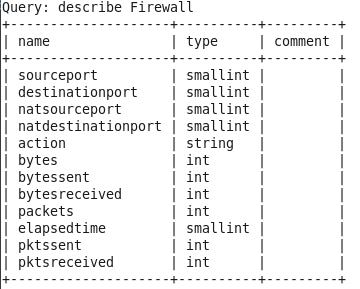
\includegraphics[width=.75\linewidth]{img/1.png}\end{figure}

\newpage

Cargamos los datos en la tabla
\begin{lstlisting}
    > LOAD DATA INPATH '/user/impala/input/log2.csv' 
      OVERWRITE INTO TABLE Firewall;
\end{lstlisting}

\begin{figure}[H]\center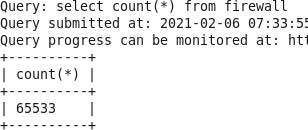
\includegraphics[width=.65\linewidth]{img/2.png}\end{figure}

Aplicamos la consulta: \textit{Obtener los 3 puertos de destino con más peticiones permitidas, mostrando este número de peticiones y el tiempo medio implicado}
\begin{lstlisting}
    > SELECT DestinationPort, COUNT(*), AVG(ElapsedTime) 
        FROM Firewall
        WHERE Action = "allow"
        GROUP BY DestinationPort
        ORDER BY 2 DESC
        LIMIT 3;
\end{lstlisting}

\begin{figure}[H]\center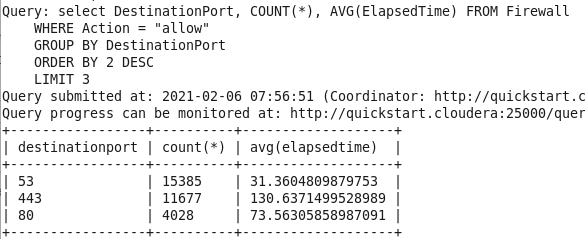
\includegraphics[width=.95\linewidth]{img/3.png}\end{figure}

\begin{itemize}
    \item En el SELECT indicamos los campos a proyectar.
    \item En el WHERE seleccionamos aquellas instancias de peticiones que el firewall ha permitido.
    \item Para poder aplicar el COUNT y el AVG, agrupamos por puertos de destino.
    \item Ordenamos en orden decreciente por la cuenta de peticiones y con el LIMIT nos quedamos con los 3 puertos pedidos.
\end{itemize}

    \setlength{\parskip}{1em}
    
    % ==============================================================================
    
    \newpage
    % \nocite{*}
    % \bibliography{bibliografia}
	% \bibliographystyle{plain}
\end{document}

% ==============================================================================
% ==============================================================================